\documentclass[1p]{elsarticle_modified}
%\bibliographystyle{elsarticle-num}

%\usepackage[colorlinks]{hyperref}
%\usepackage{abbrmath_seonhwa} %\Abb, \Ascr, \Acal ,\Abf, \Afrak
\usepackage{amsfonts}
\usepackage{amssymb}
\usepackage{amsmath}
\usepackage{amsthm}
\usepackage{scalefnt}
\usepackage{amsbsy}
\usepackage{kotex}
\usepackage{caption}
\usepackage{subfig}
\usepackage{color}
\usepackage{graphicx}
\usepackage{xcolor} %% white, black, red, green, blue, cyan, magenta, yellow
\usepackage{float}
\usepackage{setspace}
\usepackage{hyperref}

\usepackage{tikz}
\usetikzlibrary{arrows}

\usepackage{multirow}
\usepackage{array} % fixed length table
\usepackage{hhline}

%%%%%%%%%%%%%%%%%%%%%
\makeatletter
\renewcommand*\env@matrix[1][\arraystretch]{%
	\edef\arraystretch{#1}%
	\hskip -\arraycolsep
	\let\@ifnextchar\new@ifnextchar
	\array{*\c@MaxMatrixCols c}}
\makeatother %https://tex.stackexchange.com/questions/14071/how-can-i-increase-the-line-spacing-in-a-matrix
%%%%%%%%%%%%%%%

\usepackage[normalem]{ulem}

\newcommand{\msout}[1]{\ifmmode\text{\sout{\ensuremath{#1}}}\else\sout{#1}\fi}
%SOURCE: \msout is \stkout macro in https://tex.stackexchange.com/questions/20609/strikeout-in-math-mode

\newcommand{\cancel}[1]{
	\ifmmode
	{\color{red}\msout{#1}}
	\else
	{\color{red}\sout{#1}}
	\fi
}

\newcommand{\add}[1]{
	{\color{blue}\uwave{#1}}
}

\newcommand{\replace}[2]{
	\ifmmode
	{\color{red}\msout{#1}}{\color{blue}\uwave{#2}}
	\else
	{\color{red}\sout{#1}}{\color{blue}\uwave{#2}}
	\fi
}

\newcommand{\Sol}{\mathcal{S}} %segment
\newcommand{\D}{D} %diagram
\newcommand{\A}{\mathcal{A}} %arc


%%%%%%%%%%%%%%%%%%%%%%%%%%%%%5 test

\def\sl{\operatorname{\textup{SL}}(2,\Cbb)}
\def\psl{\operatorname{\textup{PSL}}(2,\Cbb)}
\def\quan{\mkern 1mu \triangleright \mkern 1mu}

\theoremstyle{definition}
\newtheorem{thm}{Theorem}[section]
\newtheorem{prop}[thm]{Proposition}
\newtheorem{lem}[thm]{Lemma}
\newtheorem{ques}[thm]{Question}
\newtheorem{cor}[thm]{Corollary}
\newtheorem{defn}[thm]{Definition}
\newtheorem{exam}[thm]{Example}
\newtheorem{rmk}[thm]{Remark}
\newtheorem{alg}[thm]{Algorithm}

\newcommand{\I}{\sqrt{-1}}
\begin{document}

%\begin{frontmatter}
%
%\title{Boundary parabolic representations of knots up to 8 crossings}
%
%%% Group authors per affiliation:
%\author{Yunhi Cho} 
%\address{Department of Mathematics, University of Seoul, Seoul, Korea}
%\ead{yhcho@uos.ac.kr}
%
%
%\author{Seonhwa Kim} %\fnref{s_kim}}
%\address{Center for Geometry and Physics, Institute for Basic Science, Pohang, 37673, Korea}
%\ead{ryeona17@ibs.re.kr}
%
%\author{Hyuk Kim}
%\address{Department of Mathematical Sciences, Seoul National University, Seoul 08826, Korea}
%\ead{hyukkim@snu.ac.kr}
%
%\author{Seokbeom Yoon}
%\address{Department of Mathematical Sciences, Seoul National University, Seoul, 08826,  Korea}
%\ead{sbyoon15@snu.ac.kr}
%
%\begin{abstract}
%We find all boundary parabolic representation of knots up to 8 crossings.
%
%\end{abstract}
%\begin{keyword}
%    \MSC[2010] 57M25 
%\end{keyword}
%
%\end{frontmatter}

%\linenumbers
%\tableofcontents
%
\newcommand\colored[1]{\textcolor{white}{\rule[-0.35ex]{0.8em}{1.4ex}}\kern-0.8em\color{red} #1}%
%\newcommand\colored[1]{\textcolor{white}{ #1}\kern-2.17ex	\textcolor{white}{ #1}\kern-1.81ex	\textcolor{white}{ #1}\kern-2.15ex\color{red}#1	}

{\Large $\underline{12n_{0452}~(K12n_{0452})}$}

\setlength{\tabcolsep}{10pt}
\renewcommand{\arraystretch}{1.6}
\vspace{1cm}\begin{tabular}{m{100pt}>{\centering\arraybackslash}m{274pt}}
\multirow{5}{120pt}{
	\centering
	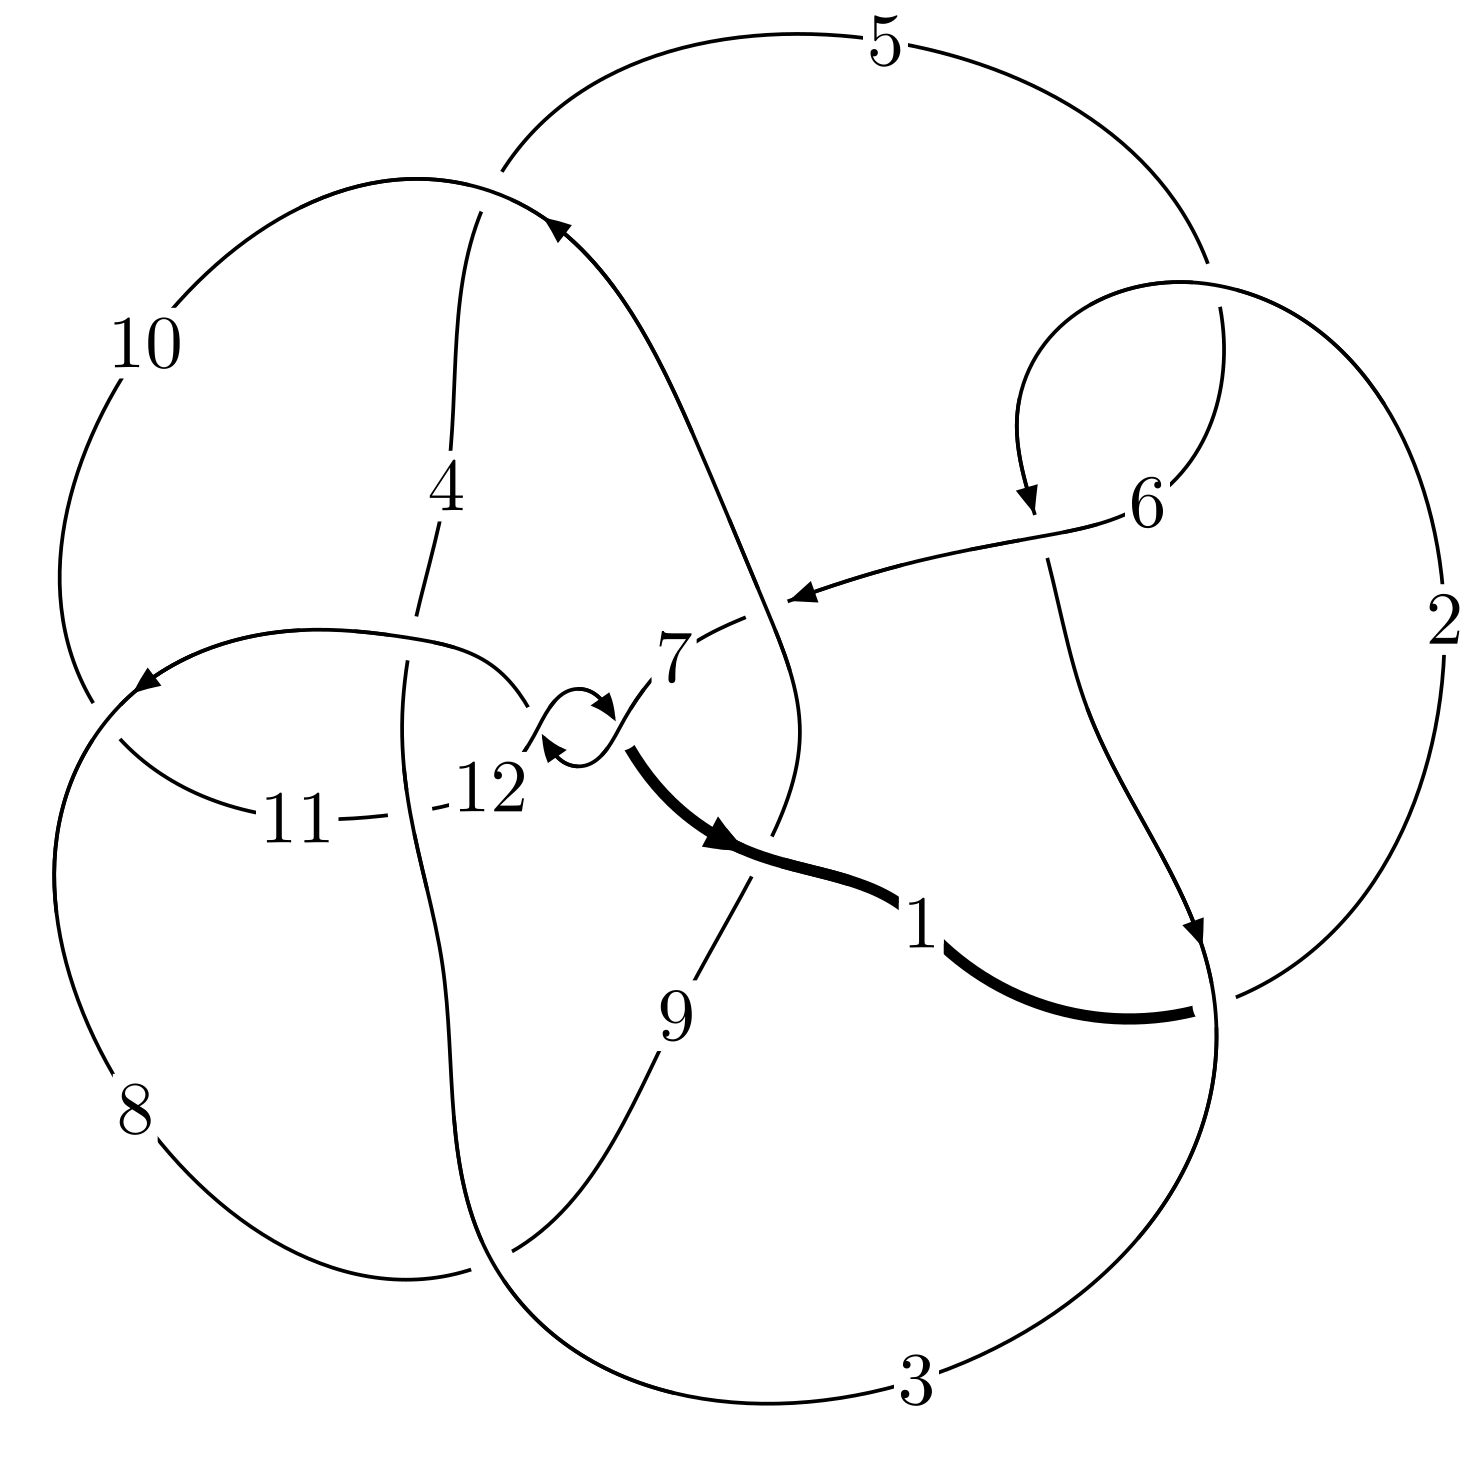
\includegraphics[width=112pt]{../../../GIT/diagram.site/Diagrams/png/2541_12n_0452.png}\\
\ \ \ A knot diagram\footnotemark}&
\allowdisplaybreaks
\textbf{Linearized knot diagam} \\
\cline{2-2}
 &
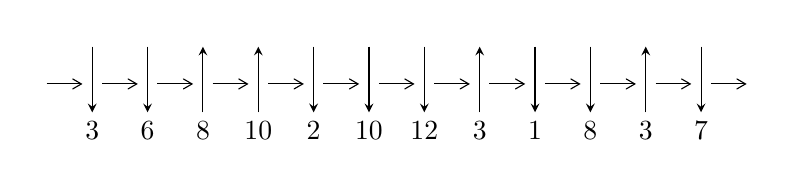
\begin{tikzpicture}[x=20pt, y=17pt]
	% nodes
	\node (C0) at (0, 0) {};
	\node (C1) at (1, 0) {};
	\node (C1U) at (1, +1) {};
	\node (C1D) at (1, -1) {3};

	\node (C2) at (2, 0) {};
	\node (C2U) at (2, +1) {};
	\node (C2D) at (2, -1) {6};

	\node (C3) at (3, 0) {};
	\node (C3U) at (3, +1) {};
	\node (C3D) at (3, -1) {8};

	\node (C4) at (4, 0) {};
	\node (C4U) at (4, +1) {};
	\node (C4D) at (4, -1) {10};

	\node (C5) at (5, 0) {};
	\node (C5U) at (5, +1) {};
	\node (C5D) at (5, -1) {2};

	\node (C6) at (6, 0) {};
	\node (C6U) at (6, +1) {};
	\node (C6D) at (6, -1) {10};

	\node (C7) at (7, 0) {};
	\node (C7U) at (7, +1) {};
	\node (C7D) at (7, -1) {12};

	\node (C8) at (8, 0) {};
	\node (C8U) at (8, +1) {};
	\node (C8D) at (8, -1) {3};

	\node (C9) at (9, 0) {};
	\node (C9U) at (9, +1) {};
	\node (C9D) at (9, -1) {1};

	\node (C10) at (10, 0) {};
	\node (C10U) at (10, +1) {};
	\node (C10D) at (10, -1) {8};

	\node (C11) at (11, 0) {};
	\node (C11U) at (11, +1) {};
	\node (C11D) at (11, -1) {3};

	\node (C12) at (12, 0) {};
	\node (C12U) at (12, +1) {};
	\node (C12D) at (12, -1) {7};
	\node (C13) at (13, 0) {};

	% arrows
	\draw[->,>={angle 60}]
	(C0) edge (C1) (C1) edge (C2) (C2) edge (C3) (C3) edge (C4) (C4) edge (C5) (C5) edge (C6) (C6) edge (C7) (C7) edge (C8) (C8) edge (C9) (C9) edge (C10) (C10) edge (C11) (C11) edge (C12) (C12) edge (C13) ;	\draw[->,>=stealth]
	(C1U) edge (C1D) (C2U) edge (C2D) (C3D) edge (C3U) (C4D) edge (C4U) (C5U) edge (C5D) (C6U) edge (C6D) (C7U) edge (C7D) (C8D) edge (C8U) (C9U) edge (C9D) (C10U) edge (C10D) (C11D) edge (C11U) (C12U) edge (C12D) ;
	\end{tikzpicture} \\
\hhline{~~} \\& 
\textbf{Solving Sequence} \\ \cline{2-2} 
 &
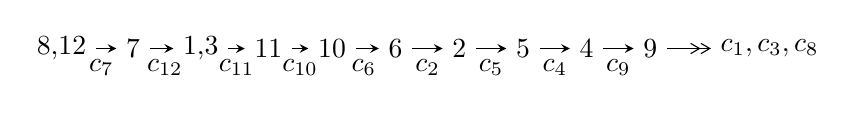
\begin{tikzpicture}[x=23pt, y=7pt]
	% node
	\node (A0) at (-1/8, 0) {8,12};
	\node (A1) at (1, 0) {7};
	\node (A2) at (33/16, 0) {1,3};
	\node (A3) at (25/8, 0) {11};
	\node (A4) at (33/8, 0) {10};
	\node (A5) at (41/8, 0) {6};
	\node (A6) at (49/8, 0) {2};
	\node (A7) at (57/8, 0) {5};
	\node (A8) at (65/8, 0) {4};
	\node (A9) at (73/8, 0) {9};
	\node (C1) at (1/2, -1) {$c_{7}$};
	\node (C2) at (3/2, -1) {$c_{12}$};
	\node (C3) at (21/8, -1) {$c_{11}$};
	\node (C4) at (29/8, -1) {$c_{10}$};
	\node (C5) at (37/8, -1) {$c_{6}$};
	\node (C6) at (45/8, -1) {$c_{2}$};
	\node (C7) at (53/8, -1) {$c_{5}$};
	\node (C8) at (61/8, -1) {$c_{4}$};
	\node (C9) at (69/8, -1) {$c_{9}$};
	\node (A10) at (11, 0) {$c_{1},c_{3},c_{8}$};

	% edge
	\draw[->,>=stealth]	
	(A0) edge (A1) (A1) edge (A2) (A2) edge (A3) (A3) edge (A4) (A4) edge (A5) (A5) edge (A6) (A6) edge (A7) (A7) edge (A8) (A8) edge (A9) ;
	\draw[->>,>={angle 60}]	
	(A9) edge (A10);
\end{tikzpicture} \\ 

\end{tabular} \\

\footnotetext{
The image of knot diagram is generated by the software ``\textbf{Draw programme}" developed by Andrew Bartholomew(\url{http://www.layer8.co.uk/maths/draw/index.htm\#Running-draw}), where we modified some parts for our purpose(\url{https://github.com/CATsTAILs/LinksPainter}).
}\phantom \\ \newline 
\centering \textbf{Ideals for irreducible components\footnotemark of $X_{\text{par}}$} 
 
\begin{align*}
I^u_{1}&=\langle 
-2 u^{19}+19 u^{18}+\cdots+4 b-12,\;3 u^{19}-20 u^{18}+\cdots+32 a-80,\;u^{20}-12 u^{19}+\cdots+288 u-32\rangle \\
I^u_{2}&=\langle 
-145388409 a^9 u-416262498 a^8 u+\cdots-5046614442 a-113580331,\\
\phantom{I^u_{2}}&\phantom{= \langle  }- a^9 u+4 a^8 u+\cdots+2 a+1,\;u^2+u+1\rangle \\
I^u_{3}&=\langle 
2 u^{12}+2 u^{11}+8 u^{10}+5 u^9+15 u^8- u^7+13 u^6-10 u^5+5 u^4-11 u^3+2 u^2+b-3 u,\\
\phantom{I^u_{3}}&\phantom{= \langle  }2 u^{11}+2 u^{10}+8 u^9+5 u^8+15 u^7- u^6+13 u^5-10 u^4+5 u^3-11 u^2+a+2 u-3,\\
\phantom{I^u_{3}}&\phantom{= \langle  }u^{13}+u^{12}+5 u^{11}+4 u^{10}+12 u^9+4 u^8+15 u^7-2 u^6+8 u^5-8 u^4-6 u^2-2 u-1\rangle \\
\\
\end{align*}
\raggedright * 3 irreducible components of $\dim_{\mathbb{C}}=0$, with total 53 representations.\\
\footnotetext{All coefficients of polynomials are rational numbers. But the coefficients are sometimes approximated in decimal forms when there is not enough margin.}
\newpage
\renewcommand{\arraystretch}{1}
\centering \section*{I. $I^u_{1}= \langle -2 u^{19}+19 u^{18}+\cdots+4 b-12,\;3 u^{19}-20 u^{18}+\cdots+32 a-80,\;u^{20}-12 u^{19}+\cdots+288 u-32 \rangle$}
\flushleft \textbf{(i) Arc colorings}\\
\begin{tabular}{m{7pt} m{180pt} m{7pt} m{180pt} }
\flushright $a_{8}=$&$\begin{pmatrix}1\\0\end{pmatrix}$ \\
\flushright $a_{12}=$&$\begin{pmatrix}0\\u\end{pmatrix}$ \\
\flushright $a_{7}=$&$\begin{pmatrix}1\\- u^2\end{pmatrix}$ \\
\flushright $a_{1}=$&$\begin{pmatrix}- u\\u^3+u\end{pmatrix}$ \\
\flushright $a_{3}=$&$\begin{pmatrix}-\frac{3}{32} u^{19}+\frac{5}{8} u^{18}+\cdots-\frac{23}{2} u+\frac{5}{2}\\\frac{1}{2} u^{19}-\frac{19}{4} u^{18}+\cdots-\frac{59}{2} u+3\end{pmatrix}$ \\
\flushright $a_{11}=$&$\begin{pmatrix}-\frac{19}{32} u^{19}+\frac{105}{16} u^{18}+\cdots+\frac{267}{2} u-16\\\frac{9}{16} u^{19}-\frac{51}{8} u^{18}+\cdots-154 u+19\end{pmatrix}$ \\
\flushright $a_{10}=$&$\begin{pmatrix}-\frac{1}{32} u^{19}+\frac{3}{16} u^{18}+\cdots-\frac{41}{2} u+3\\\frac{9}{16} u^{19}-\frac{51}{8} u^{18}+\cdots-154 u+19\end{pmatrix}$ \\
\flushright $a_{6}=$&$\begin{pmatrix}-\frac{1}{32} u^{19}-\frac{1}{8} u^{18}+\cdots-16 u+2\\-\frac{1}{2} u^{19}+\frac{45}{8} u^{18}+\cdots+218 u-29\end{pmatrix}$ \\
\flushright $a_{2}=$&$\begin{pmatrix}-\frac{13}{32} u^{19}+\frac{71}{16} u^{18}+\cdots+\frac{241}{2} u-15\\\frac{7}{16} u^{19}-\frac{37}{8} u^{18}+\cdots-101 u+13\end{pmatrix}$ \\
\flushright $a_{5}=$&$\begin{pmatrix}\frac{1}{16} u^{19}-\frac{27}{16} u^{18}+\cdots-\frac{167}{4} u+\frac{7}{2}\\-\frac{3}{16} u^{19}+\frac{19}{8} u^{18}+\cdots+\frac{371}{2} u-24\end{pmatrix}$ \\
\flushright $a_{4}=$&$\begin{pmatrix}-\frac{13}{32} u^{19}+\frac{33}{8} u^{18}+\cdots+41 u-\frac{11}{2}\\-\frac{1}{2} u^{19}+\frac{19}{4} u^{18}+\cdots+\frac{59}{2} u-3\end{pmatrix}$ \\
\flushright $a_{9}=$&$\begin{pmatrix}\frac{19}{32} u^{19}-\frac{105}{16} u^{18}+\cdots-\frac{267}{2} u+17\\-\frac{9}{16} u^{19}+\frac{51}{8} u^{18}+\cdots+155 u-19\end{pmatrix}$\\&\end{tabular}
\flushleft \textbf{(ii) Obstruction class $= -1$}\\~\\
\flushleft \textbf{(iii) Cusp Shapes $= \frac{7}{4} u^{19}-20 u^{18}+\frac{491}{4} u^{17}-517 u^{16}+\frac{6595}{4} u^{15}-\frac{8353}{2} u^{14}+\frac{34489}{4} u^{13}-\frac{58707}{4} u^{12}+\frac{82427}{4} u^{11}-\frac{47101}{2} u^{10}+\frac{42177}{2} u^9-13237 u^8+3090 u^7+\frac{19739}{4} u^6-\frac{32253}{4} u^5+\frac{27135}{4} u^4-\frac{7505}{2} u^3+1346 u^2-268 u+14$}\\~\\
\newpage\renewcommand{\arraystretch}{1}
\flushleft \textbf{(iv) u-Polynomials at the component}\newline \\
\begin{tabular}{m{50pt}|m{274pt}}
Crossings & \hspace{64pt}u-Polynomials at each crossing \\
\hline $$\begin{aligned}c_{1}\end{aligned}$$&$\begin{aligned}
&u^{20}+8 u^{19}+\cdots+140 u+16
\end{aligned}$\\
\hline $$\begin{aligned}c_{2},c_{5}\end{aligned}$$&$\begin{aligned}
&u^{20}+8 u^{19}+\cdots-14 u-4
\end{aligned}$\\
\hline $$\begin{aligned}c_{3},c_{4},c_{8}\\c_{11}\end{aligned}$$&$\begin{aligned}
&u^{20}+13 u^{18}+\cdots-2 u+1
\end{aligned}$\\
\hline $$\begin{aligned}c_{6},c_{9}\end{aligned}$$&$\begin{aligned}
&u^{20}- u^{19}+\cdots+8 u-1
\end{aligned}$\\
\hline $$\begin{aligned}c_{7},c_{12}\end{aligned}$$&$\begin{aligned}
&u^{20}+12 u^{19}+\cdots-288 u-32
\end{aligned}$\\
\hline $$\begin{aligned}c_{10}\end{aligned}$$&$\begin{aligned}
&u^{20}-14 u^{19}+\cdots+92 u-16
\end{aligned}$\\
\hline
\end{tabular}\\~\\
\newpage\renewcommand{\arraystretch}{1}
\flushleft \textbf{(v) Riley Polynomials at the component}\newline \\
\begin{tabular}{m{50pt}|m{274pt}}
Crossings & \hspace{64pt}Riley Polynomials at each crossing \\
\hline $$\begin{aligned}c_{1}\end{aligned}$$&$\begin{aligned}
&y^{20}+12 y^{19}+\cdots+144 y+256
\end{aligned}$\\
\hline $$\begin{aligned}c_{2},c_{5}\end{aligned}$$&$\begin{aligned}
&y^{20}-8 y^{19}+\cdots-140 y+16
\end{aligned}$\\
\hline $$\begin{aligned}c_{3},c_{4},c_{8}\\c_{11}\end{aligned}$$&$\begin{aligned}
&y^{20}+26 y^{19}+\cdots-6 y+1
\end{aligned}$\\
\hline $$\begin{aligned}c_{6},c_{9}\end{aligned}$$&$\begin{aligned}
&y^{20}+15 y^{19}+\cdots-44 y+1
\end{aligned}$\\
\hline $$\begin{aligned}c_{7},c_{12}\end{aligned}$$&$\begin{aligned}
&y^{20}+10 y^{19}+\cdots-2560 y+1024
\end{aligned}$\\
\hline $$\begin{aligned}c_{10}\end{aligned}$$&$\begin{aligned}
&y^{20}-2 y^{19}+\cdots+1488 y+256
\end{aligned}$\\
\hline
\end{tabular}\\~\\
\newpage\flushleft \textbf{(vi) Complex Volumes and Cusp Shapes}
$$\begin{array}{c|c|c}  
\text{Solutions to }I^u_{1}& \I (\text{vol} + \sqrt{-1}CS) & \text{Cusp shape}\\
 \hline 
\begin{aligned}
u &= \phantom{-}1.075750 + 0.527136 I \\
a &= -0.573996 - 1.042510 I \\
b &= \phantom{-}0.06793 + 1.42405 I\end{aligned}
 & -0.652295 - 0.063400 I & -3.10398 + 0.28543 I \\ \hline\begin{aligned}
u &= \phantom{-}1.075750 - 0.527136 I \\
a &= -0.573996 + 1.042510 I \\
b &= \phantom{-}0.06793 - 1.42405 I\end{aligned}
 & -0.652295 + 0.063400 I & -3.10398 - 0.28543 I \\ \hline\begin{aligned}
u &= -0.773680\phantom{ +0.000000I} \\
a &= \phantom{-}0.883116\phantom{ +0.000000I} \\
b &= \phantom{-}0.683249\phantom{ +0.000000I}\end{aligned}
 & -2.79948\phantom{ +0.000000I} & \phantom{-}5.16970\phantom{ +0.000000I} \\ \hline\begin{aligned}
u &= \phantom{-}1.220080 + 0.372661 I \\
a &= \phantom{-}0.488481 + 1.192350 I \\
b &= -0.15165 - 1.63680 I\end{aligned}
 & -2.48213 + 6.73732 I & -5.81800 - 4.44905 I \\ \hline\begin{aligned}
u &= \phantom{-}1.220080 - 0.372661 I \\
a &= \phantom{-}0.488481 - 1.192350 I \\
b &= -0.15165 + 1.63680 I\end{aligned}
 & -2.48213 - 6.73732 I & -5.81800 + 4.44905 I \\ \hline\begin{aligned}
u &= \phantom{-}0.224454 + 1.268350 I \\
a &= -0.027225 - 0.309278 I \\
b &= -0.386163 + 0.103950 I\end{aligned}
 & \phantom{-}2.15799 - 3.14030 I & \phantom{-}6.33386 + 3.02203 I \\ \hline\begin{aligned}
u &= \phantom{-}0.224454 - 1.268350 I \\
a &= -0.027225 + 0.309278 I \\
b &= -0.386163 - 0.103950 I\end{aligned}
 & \phantom{-}2.15799 + 3.14030 I & \phantom{-}6.33386 - 3.02203 I \\ \hline\begin{aligned}
u &= \phantom{-}0.641665\phantom{ +0.000000I} \\
a &= -0.577618\phantom{ +0.000000I} \\
b &= \phantom{-}0.370637\phantom{ +0.000000I}\end{aligned}
 & -1.75232\phantom{ +0.000000I} & -4.33040\phantom{ +0.000000I} \\ \hline\begin{aligned}
u &= \phantom{-}0.27440 + 1.41304 I \\
a &= \phantom{-}0.552394 - 0.086578 I \\
b &= -0.273914 - 0.756798 I\end{aligned}
 & \phantom{-}5.72955 - 3.97634 I & -2.60990 + 3.53536 I \\ \hline\begin{aligned}
u &= \phantom{-}0.27440 - 1.41304 I \\
a &= \phantom{-}0.552394 + 0.086578 I \\
b &= -0.273914 + 0.756798 I\end{aligned}
 & \phantom{-}5.72955 + 3.97634 I & -2.60990 - 3.53536 I\\
 \hline 
 \end{array}$$\newpage$$\begin{array}{c|c|c}  
\text{Solutions to }I^u_{1}& \I (\text{vol} + \sqrt{-1}CS) & \text{Cusp shape}\\
 \hline 
\begin{aligned}
u &= \phantom{-}0.75896 + 1.24508 I \\
a &= -0.712912 - 0.941128 I \\
b &= -0.63071 + 1.60191 I\end{aligned}
 & \phantom{-}1.64002 - 6.67897 I & -2.46195 + 3.53003 I \\ \hline\begin{aligned}
u &= \phantom{-}0.75896 - 1.24508 I \\
a &= -0.712912 + 0.941128 I \\
b &= -0.63071 - 1.60191 I\end{aligned}
 & \phantom{-}1.64002 + 6.67897 I & -2.46195 - 3.53003 I \\ \hline\begin{aligned}
u &= \phantom{-}0.378434 + 0.367449 I \\
a &= -0.582962 - 0.854221 I \\
b &= -0.093271 + 0.537475 I\end{aligned}
 & -0.254529 - 1.078120 I & -3.77931 + 6.22924 I \\ \hline\begin{aligned}
u &= \phantom{-}0.378434 - 0.367449 I \\
a &= -0.582962 + 0.854221 I \\
b &= -0.093271 - 0.537475 I\end{aligned}
 & -0.254529 + 1.078120 I & -3.77931 - 6.22924 I \\ \hline\begin{aligned}
u &= \phantom{-}0.73237 + 1.30566 I \\
a &= \phantom{-}0.793219 + 0.921154 I \\
b &= \phantom{-}0.62179 - 1.71030 I\end{aligned}
 & \phantom{-}0.48491 - 13.65130 I & -3.87240 + 7.23711 I \\ \hline\begin{aligned}
u &= \phantom{-}0.73237 - 1.30566 I \\
a &= \phantom{-}0.793219 - 0.921154 I \\
b &= \phantom{-}0.62179 + 1.71030 I\end{aligned}
 & \phantom{-}0.48491 + 13.65130 I & -3.87240 - 7.23711 I \\ \hline\begin{aligned}
u &= \phantom{-}0.24241 + 1.52074 I \\
a &= -0.616057 - 0.104390 I \\
b &= -0.009409 + 0.962170 I\end{aligned}
 & \phantom{-}4.41718 + 1.57291 I & -2.59421 - 1.48846 I \\ \hline\begin{aligned}
u &= \phantom{-}0.24241 - 1.52074 I \\
a &= -0.616057 + 0.104390 I \\
b &= -0.009409 - 0.962170 I\end{aligned}
 & \phantom{-}4.41718 - 1.57291 I & -2.59421 + 1.48846 I \\ \hline\begin{aligned}
u &= \phantom{-}1.15915 + 1.09993 I \\
a &= \phantom{-}0.526308 + 0.853253 I \\
b &= \phantom{-}0.32845 - 1.56795 I\end{aligned}
 & -7.94232 - 4.19743 I & -2.01377 + 4.62761 I \\ \hline\begin{aligned}
u &= \phantom{-}1.15915 - 1.09993 I \\
a &= \phantom{-}0.526308 - 0.853253 I \\
b &= \phantom{-}0.32845 + 1.56795 I\end{aligned}
 & -7.94232 + 4.19743 I & -2.01377 - 4.62761 I\\
 \hline 
 \end{array}$$\newpage\newpage\renewcommand{\arraystretch}{1}
\centering \section*{II. $I^u_{2}= \langle -1.45\times10^{8} a^{9} u-4.16\times10^{8} a^{8} u+\cdots-5.05\times10^{9} a-1.14\times10^{8},\;- a^9 u+4 a^8 u+\cdots+2 a+1,\;u^2+u+1 \rangle$}
\flushleft \textbf{(i) Arc colorings}\\
\begin{tabular}{m{7pt} m{180pt} m{7pt} m{180pt} }
\flushright $a_{8}=$&$\begin{pmatrix}1\\0\end{pmatrix}$ \\
\flushright $a_{12}=$&$\begin{pmatrix}0\\u\end{pmatrix}$ \\
\flushright $a_{7}=$&$\begin{pmatrix}1\\u+1\end{pmatrix}$ \\
\flushright $a_{1}=$&$\begin{pmatrix}- u\\u+1\end{pmatrix}$ \\
\flushright $a_{3}=$&$\begin{pmatrix}a\\0.161928 a^{9} u+0.463617 a^{8} u+\cdots+5.62073 a+0.126501\end{pmatrix}$ \\
\flushright $a_{11}=$&$\begin{pmatrix}- a^2 u\\0.0874157 a^{9} u-0.164877 a^{8} u+\cdots-1.57349 a-2.70031\end{pmatrix}$ \\
\flushright $a_{10}=$&$\begin{pmatrix}0.0874157 a^{9} u-0.164877 a^{8} u+\cdots-1.57349 a-2.70031\\0.0874157 a^{9} u-0.164877 a^{8} u+\cdots-1.57349 a-2.70031\end{pmatrix}$ \\
\flushright $a_{6}=$&$\begin{pmatrix}0.0351466 a^{9} u-0.131650 a^{8} u+\cdots-2.53636 a+0.218613\\-0.00781644 a^{9} u+0.156367 a^{8} u+\cdots-0.328653 a+1.97905\end{pmatrix}$ \\
\flushright $a_{2}=$&$\begin{pmatrix}0.0874157 a^{9} u-0.164877 a^{8} u+\cdots-1.57349 a-2.70031\\0.275733 a^{9} u+0.677652 a^{8} u+\cdots+2.30695 a-1.97416\end{pmatrix}$ \\
\flushright $a_{5}=$&$\begin{pmatrix}0.0777622 a^{9} u-0.0954980 a^{8} u+\cdots-6.08282 a-0.886513\\0.0777622 a^{9} u-0.0954980 a^{8} u+\cdots-5.08282 a-0.886513\end{pmatrix}$ \\
\flushright $a_{4}=$&$\begin{pmatrix}-0.161928 a^{9} u-0.463617 a^{8} u+\cdots-6.62073 a-0.126501\\-0.161928 a^{9} u-0.463617 a^{8} u+\cdots-5.62073 a-0.126501\end{pmatrix}$ \\
\flushright $a_{9}=$&$\begin{pmatrix}-0.181574 a^{9} u-0.256387 a^{8} u+\cdots-0.366731 a+2.33724\\0.0806728 a^{9} u-0.751019 a^{8} u+\cdots-5.08719 a-5.76370\end{pmatrix}$\\&\end{tabular}
\flushleft \textbf{(ii) Obstruction class $= -1$}\\~\\
\flushleft \textbf{(iii) Cusp Shapes $= \frac{510421912}{897858103} a^9 u+\frac{905299596}{897858103} a^8 u+\cdots+\frac{3135128908}{897858103} a-\frac{6259589598}{897858103}$}\\~\\
\newpage\renewcommand{\arraystretch}{1}
\flushleft \textbf{(iv) u-Polynomials at the component}\newline \\
\begin{tabular}{m{50pt}|m{274pt}}
Crossings & \hspace{64pt}u-Polynomials at each crossing \\
\hline $$\begin{aligned}c_{1}\end{aligned}$$&$\begin{aligned}
&(u^5+u^4+4 u^3+3 u^2+3 u+1)^4
\end{aligned}$\\
\hline $$\begin{aligned}c_{2},c_{5}\end{aligned}$$&$\begin{aligned}
&(u^5- u^4+u^2+u-1)^4
\end{aligned}$\\
\hline $$\begin{aligned}c_{3},c_{4},c_{8}\\c_{11}\end{aligned}$$&$\begin{aligned}
&u^{20}+u^{19}+\cdots+16 u+91
\end{aligned}$\\
\hline $$\begin{aligned}c_{6},c_{9}\end{aligned}$$&$\begin{aligned}
&u^{20}+3 u^{19}+\cdots+480 u+193
\end{aligned}$\\
\hline $$\begin{aligned}c_{7},c_{12}\end{aligned}$$&$\begin{aligned}
&(u^2- u+1)^{10}
\end{aligned}$\\
\hline $$\begin{aligned}c_{10}\end{aligned}$$&$\begin{aligned}
&(u^5+3 u^4-5 u^2- u+3)^4
\end{aligned}$\\
\hline
\end{tabular}\\~\\
\newpage\renewcommand{\arraystretch}{1}
\flushleft \textbf{(v) Riley Polynomials at the component}\newline \\
\begin{tabular}{m{50pt}|m{274pt}}
Crossings & \hspace{64pt}Riley Polynomials at each crossing \\
\hline $$\begin{aligned}c_{1}\end{aligned}$$&$\begin{aligned}
&(y^5+7 y^4+16 y^3+13 y^2+3 y-1)^4
\end{aligned}$\\
\hline $$\begin{aligned}c_{2},c_{5}\end{aligned}$$&$\begin{aligned}
&(y^5- y^4+4 y^3-3 y^2+3 y-1)^4
\end{aligned}$\\
\hline $$\begin{aligned}c_{3},c_{4},c_{8}\\c_{11}\end{aligned}$$&$\begin{aligned}
&y^{20}+15 y^{19}+\cdots+124596 y+8281
\end{aligned}$\\
\hline $$\begin{aligned}c_{6},c_{9}\end{aligned}$$&$\begin{aligned}
&y^{20}+11 y^{19}+\cdots-106108 y+37249
\end{aligned}$\\
\hline $$\begin{aligned}c_{7},c_{12}\end{aligned}$$&$\begin{aligned}
&(y^2+y+1)^{10}
\end{aligned}$\\
\hline $$\begin{aligned}c_{10}\end{aligned}$$&$\begin{aligned}
&(y^5-9 y^4+28 y^3-43 y^2+31 y-9)^4
\end{aligned}$\\
\hline
\end{tabular}\\~\\
\newpage\flushleft \textbf{(vi) Complex Volumes and Cusp Shapes}
$$\begin{array}{c|c|c}  
\text{Solutions to }I^u_{2}& \I (\text{vol} + \sqrt{-1}CS) & \text{Cusp shape}\\
 \hline 
\begin{aligned}
u &= -0.500000 + 0.866025 I \\
a &= \phantom{-}0.667123 - 0.865495 I \\
b &= -0.23410 + 1.65564 I\end{aligned}
 & -3.11500 - 0.18409 I & -5.11432 + 0.75879 I \\ \hline\begin{aligned}
u &= -0.500000 + 0.866025 I \\
a &= \phantom{-}0.487783 - 0.467051 I \\
b &= \phantom{-}1.65437 - 0.13929 I\end{aligned}
 & \phantom{-}6.02349 + 5.36163 I & -4.08126 - 5.82638 I \\ \hline\begin{aligned}
u &= -0.500000 + 0.866025 I \\
a &= \phantom{-}1.26160 - 0.72565 I \\
b &= \phantom{-}0.88139 + 1.21499 I\end{aligned}
 & -3.11500 + 4.24385 I & -5.11432 - 7.68699 I \\ \hline\begin{aligned}
u &= -0.500000 + 0.866025 I \\
a &= \phantom{-}1.20118 - 0.88684 I \\
b &= \phantom{-}0.37558 + 1.84419 I\end{aligned}
 & -5.81699 + 2.02988 I & -13.60884 - 3.46410 I \\ \hline\begin{aligned}
u &= -0.500000 + 0.866025 I \\
a &= -0.61152 + 1.37080 I \\
b &= \phantom{-}0.00237 - 1.45540 I\end{aligned}
 & -3.11500 + 4.24385 I & -5.11432 - 7.68699 I \\ \hline\begin{aligned}
u &= -0.500000 + 0.866025 I \\
a &= -0.350835 + 0.320152 I \\
b &= -1.53744 + 0.43212 I\end{aligned}
 & \phantom{-}6.02349 - 1.30186 I & -4.08126 - 1.10182 I \\ \hline\begin{aligned}
u &= -0.500000 + 0.866025 I \\
a &= -1.14295 - 1.11541 I \\
b &= \phantom{-}0.101843 + 0.463908 I\end{aligned}
 & \phantom{-}6.02349 - 1.30186 I & -4.08126 - 1.10182 I \\ \hline\begin{aligned}
u &= -0.500000 + 0.866025 I \\
a &= \phantom{-}0.94782 + 1.36308 I \\
b &= -0.160586 - 0.655958 I\end{aligned}
 & \phantom{-}6.02349 + 5.36163 I & -4.08126 - 5.82638 I \\ \hline\begin{aligned}
u &= -0.500000 + 0.866025 I \\
a &= -1.55088 + 0.62509 I \\
b &= -0.415979 - 1.010490 I\end{aligned}
 & -3.11500 - 0.18409 I & -5.11432 + 0.75879 I \\ \hline\begin{aligned}
u &= -0.500000 + 0.866025 I \\
a &= -1.40932 + 1.24736 I \\
b &= -0.16744 - 1.48368 I\end{aligned}
 & -5.81699 + 2.02988 I & -13.60884 - 3.46410 I\\
 \hline 
 \end{array}$$\newpage$$\begin{array}{c|c|c}  
\text{Solutions to }I^u_{2}& \I (\text{vol} + \sqrt{-1}CS) & \text{Cusp shape}\\
 \hline 
\begin{aligned}
u &= -0.500000 - 0.866025 I \\
a &= \phantom{-}0.667123 + 0.865495 I \\
b &= -0.23410 - 1.65564 I\end{aligned}
 & -3.11500 + 0.18409 I & -5.11432 - 0.75879 I \\ \hline\begin{aligned}
u &= -0.500000 - 0.866025 I \\
a &= \phantom{-}0.487783 + 0.467051 I \\
b &= \phantom{-}1.65437 + 0.13929 I\end{aligned}
 & \phantom{-}6.02349 - 5.36163 I & -4.08126 + 5.82638 I \\ \hline\begin{aligned}
u &= -0.500000 - 0.866025 I \\
a &= \phantom{-}1.26160 + 0.72565 I \\
b &= \phantom{-}0.88139 - 1.21499 I\end{aligned}
 & -3.11500 - 4.24385 I & -5.11432 + 7.68699 I \\ \hline\begin{aligned}
u &= -0.500000 - 0.866025 I \\
a &= \phantom{-}1.20118 + 0.88684 I \\
b &= \phantom{-}0.37558 - 1.84419 I\end{aligned}
 & -5.81699 - 2.02988 I & -13.60884 + 3.46410 I \\ \hline\begin{aligned}
u &= -0.500000 - 0.866025 I \\
a &= -0.61152 - 1.37080 I \\
b &= \phantom{-}0.00237 + 1.45540 I\end{aligned}
 & -3.11500 - 4.24385 I & -5.11432 + 7.68699 I \\ \hline\begin{aligned}
u &= -0.500000 - 0.866025 I \\
a &= -0.350835 - 0.320152 I \\
b &= -1.53744 - 0.43212 I\end{aligned}
 & \phantom{-}6.02349 + 1.30186 I & -4.08126 + 1.10182 I \\ \hline\begin{aligned}
u &= -0.500000 - 0.866025 I \\
a &= -1.14295 + 1.11541 I \\
b &= \phantom{-}0.101843 - 0.463908 I\end{aligned}
 & \phantom{-}6.02349 + 1.30186 I & -4.08126 + 1.10182 I \\ \hline\begin{aligned}
u &= -0.500000 - 0.866025 I \\
a &= \phantom{-}0.94782 - 1.36308 I \\
b &= -0.160586 + 0.655958 I\end{aligned}
 & \phantom{-}6.02349 - 5.36163 I & -4.08126 + 5.82638 I \\ \hline\begin{aligned}
u &= -0.500000 - 0.866025 I \\
a &= -1.55088 - 0.62509 I \\
b &= -0.415979 + 1.010490 I\end{aligned}
 & -3.11500 + 0.18409 I & -5.11432 - 0.75879 I \\ \hline\begin{aligned}
u &= -0.500000 - 0.866025 I \\
a &= -1.40932 - 1.24736 I \\
b &= -0.16744 + 1.48368 I\end{aligned}
 & -5.81699 - 2.02988 I & -13.60884 + 3.46410 I\\
 \hline 
 \end{array}$$\newpage\newpage\renewcommand{\arraystretch}{1}
\centering \section*{III. $I^u_{3}= \langle 2 u^{12}+2 u^{11}+\cdots+b-3 u,\;2 u^{11}+2 u^{10}+\cdots+a-3,\;u^{13}+u^{12}+\cdots-2 u-1 \rangle$}
\flushleft \textbf{(i) Arc colorings}\\
\begin{tabular}{m{7pt} m{180pt} m{7pt} m{180pt} }
\flushright $a_{8}=$&$\begin{pmatrix}1\\0\end{pmatrix}$ \\
\flushright $a_{12}=$&$\begin{pmatrix}0\\u\end{pmatrix}$ \\
\flushright $a_{7}=$&$\begin{pmatrix}1\\- u^2\end{pmatrix}$ \\
\flushright $a_{1}=$&$\begin{pmatrix}- u\\u^3+u\end{pmatrix}$ \\
\flushright $a_{3}=$&$\begin{pmatrix}-2 u^{11}-2 u^{10}+\cdots-2 u+3\\-2 u^{12}-2 u^{11}+\cdots-2 u^2+3 u\end{pmatrix}$ \\
\flushright $a_{11}=$&$\begin{pmatrix}2 u^{12}+2 u^{11}+\cdots-7 u-4\\- u^{11}- u^{10}-4 u^9-3 u^8-8 u^7- u^6-7 u^5+3 u^4- u^3+5 u^2+u+2\end{pmatrix}$ \\
\flushright $a_{10}=$&$\begin{pmatrix}2 u^{12}+u^{11}+\cdots-6 u-2\\- u^{11}- u^{10}-4 u^9-3 u^8-8 u^7- u^6-7 u^5+3 u^4- u^3+5 u^2+u+2\end{pmatrix}$ \\
\flushright $a_{6}=$&$\begin{pmatrix}-4 u^{12}-5 u^{11}+\cdots+12 u+4\\- u^{12}- u^{11}-4 u^{10}-2 u^9-7 u^8+2 u^7-5 u^6+8 u^5-2 u^4+7 u^3-2 u^2-2\end{pmatrix}$ \\
\flushright $a_{2}=$&$\begin{pmatrix}u^{12}+4 u^{10}+9 u^8-4 u^7+14 u^6-9 u^5+11 u^4-9 u^3+4 u^2-6 u-2\\- u^{12}- u^{11}-4 u^{10}-3 u^9-8 u^8- u^7-7 u^6+3 u^5- u^4+5 u^3+u^2+u+1\end{pmatrix}$ \\
\flushright $a_{5}=$&$\begin{pmatrix}-5 u^{12}-8 u^{11}+\cdots+11 u+1\\-2 u^{12}-3 u^{11}+\cdots+2 u^2-1\end{pmatrix}$ \\
\flushright $a_{4}=$&$\begin{pmatrix}-2 u^{12}-4 u^{11}+\cdots+u+3\\-2 u^{12}-2 u^{11}+\cdots-2 u^2+3 u\end{pmatrix}$ \\
\flushright $a_{9}=$&$\begin{pmatrix}2 u^{12}+2 u^{11}+\cdots-7 u-3\\- u^{11}- u^{10}-4 u^9-3 u^8-8 u^7- u^6-7 u^5+3 u^4- u^3+5 u^2+2\end{pmatrix}$\\&\end{tabular}
\flushleft \textbf{(ii) Obstruction class $= 1$}\\~\\
\flushleft \textbf{(iii) Cusp Shapes $= 3 u^{12}+8 u^{10}-6 u^9+11 u^8-25 u^7+16 u^6-32 u^5+17 u^4-21 u^3+10 u^2-6 u-3$}\\~\\
\newpage\renewcommand{\arraystretch}{1}
\flushleft \textbf{(iv) u-Polynomials at the component}\newline \\
\begin{tabular}{m{50pt}|m{274pt}}
Crossings & \hspace{64pt}u-Polynomials at each crossing \\
\hline $$\begin{aligned}c_{1}\end{aligned}$$&$\begin{aligned}
&u^{13}-7 u^{12}+\cdots+11 u-1
\end{aligned}$\\
\hline $$\begin{aligned}c_{2}\end{aligned}$$&$\begin{aligned}
&u^{13}+3 u^{12}+\cdots-3 u-1
\end{aligned}$\\
\hline $$\begin{aligned}c_{3},c_{11}\end{aligned}$$&$\begin{aligned}
&u^{13}+5 u^{11}+\cdots+2 u-1
\end{aligned}$\\
\hline $$\begin{aligned}c_{4},c_{8}\end{aligned}$$&$\begin{aligned}
&u^{13}+5 u^{11}+\cdots+2 u+1
\end{aligned}$\\
\hline $$\begin{aligned}c_{5}\end{aligned}$$&$\begin{aligned}
&u^{13}-3 u^{12}+\cdots-3 u+1
\end{aligned}$\\
\hline $$\begin{aligned}c_{6},c_{9}\end{aligned}$$&$\begin{aligned}
&u^{13}- u^{12}+\cdots+4 u-1
\end{aligned}$\\
\hline $$\begin{aligned}c_{7}\end{aligned}$$&$\begin{aligned}
&u^{13}+u^{12}+\cdots-2 u-1
\end{aligned}$\\
\hline $$\begin{aligned}c_{10}\end{aligned}$$&$\begin{aligned}
&u^{13}+9 u^{12}+\cdots+37 u+13
\end{aligned}$\\
\hline $$\begin{aligned}c_{12}\end{aligned}$$&$\begin{aligned}
&u^{13}- u^{12}+\cdots-2 u+1
\end{aligned}$\\
\hline
\end{tabular}\\~\\
\newpage\renewcommand{\arraystretch}{1}
\flushleft \textbf{(v) Riley Polynomials at the component}\newline \\
\begin{tabular}{m{50pt}|m{274pt}}
Crossings & \hspace{64pt}Riley Polynomials at each crossing \\
\hline $$\begin{aligned}c_{1}\end{aligned}$$&$\begin{aligned}
&y^{13}+5 y^{12}+\cdots+3 y-1
\end{aligned}$\\
\hline $$\begin{aligned}c_{2},c_{5}\end{aligned}$$&$\begin{aligned}
&y^{13}-7 y^{12}+\cdots+11 y-1
\end{aligned}$\\
\hline $$\begin{aligned}c_{3},c_{4},c_{8}\\c_{11}\end{aligned}$$&$\begin{aligned}
&y^{13}+10 y^{12}+\cdots-8 y-1
\end{aligned}$\\
\hline $$\begin{aligned}c_{6},c_{9}\end{aligned}$$&$\begin{aligned}
&y^{13}+7 y^{12}+\cdots-6 y-1
\end{aligned}$\\
\hline $$\begin{aligned}c_{7},c_{12}\end{aligned}$$&$\begin{aligned}
&y^{13}+9 y^{12}+\cdots-8 y-1
\end{aligned}$\\
\hline $$\begin{aligned}c_{10}\end{aligned}$$&$\begin{aligned}
&y^{13}-13 y^{12}+\cdots+823 y-169
\end{aligned}$\\
\hline
\end{tabular}\\~\\
\newpage\flushleft \textbf{(vi) Complex Volumes and Cusp Shapes}
$$\begin{array}{c|c|c}  
\text{Solutions to }I^u_{3}& \I (\text{vol} + \sqrt{-1}CS) & \text{Cusp shape}\\
 \hline 
\begin{aligned}
u &= -0.455315 + 0.926259 I \\
a &= \phantom{-}1.30401 - 0.92398 I \\
b &= \phantom{-}0.26211 + 1.62856 I\end{aligned}
 & -5.10038 + 1.80525 I & -0.685652 + 0.373124 I \\ \hline\begin{aligned}
u &= -0.455315 - 0.926259 I \\
a &= \phantom{-}1.30401 + 0.92398 I \\
b &= \phantom{-}0.26211 - 1.62856 I\end{aligned}
 & -5.10038 - 1.80525 I & -0.685652 - 0.373124 I \\ \hline\begin{aligned}
u &= \phantom{-}0.330629 + 1.050710 I \\
a &= \phantom{-}0.526104 - 0.756260 I \\
b &= \phantom{-}0.968558 + 0.302743 I\end{aligned}
 & \phantom{-}7.37935 + 2.09783 I & \phantom{-}1.85932 - 2.29421 I \\ \hline\begin{aligned}
u &= \phantom{-}0.330629 - 1.050710 I \\
a &= \phantom{-}0.526104 + 0.756260 I \\
b &= \phantom{-}0.968558 - 0.302743 I\end{aligned}
 & \phantom{-}7.37935 - 2.09783 I & \phantom{-}1.85932 + 2.29421 I \\ \hline\begin{aligned}
u &= \phantom{-}0.261606 + 1.120690 I \\
a &= -0.257704 + 0.773845 I \\
b &= -0.934657 - 0.086363 I\end{aligned}
 & \phantom{-}7.75893 - 4.58141 I & \phantom{-}1.77723 + 3.45534 I \\ \hline\begin{aligned}
u &= \phantom{-}0.261606 - 1.120690 I \\
a &= -0.257704 - 0.773845 I \\
b &= -0.934657 + 0.086363 I\end{aligned}
 & \phantom{-}7.75893 + 4.58141 I & \phantom{-}1.77723 - 3.45534 I \\ \hline\begin{aligned}
u &= \phantom{-}0.821318\phantom{ +0.000000I} \\
a &= -0.679855\phantom{ +0.000000I} \\
b &= -0.558377\phantom{ +0.000000I}\end{aligned}
 & -3.20028\phantom{ +0.000000I} & -15.7750\phantom{ +0.000000I} \\ \hline\begin{aligned}
u &= \phantom{-}0.187185 + 1.333980 I \\
a &= \phantom{-}0.289656 + 0.057723 I \\
b &= -0.022783 + 0.397202 I\end{aligned}
 & \phantom{-}1.68403 - 3.14745 I & -11.16043 + 3.23588 I \\ \hline\begin{aligned}
u &= \phantom{-}0.187185 - 1.333980 I \\
a &= \phantom{-}0.289656 - 0.057723 I \\
b &= -0.022783 - 0.397202 I\end{aligned}
 & \phantom{-}1.68403 + 3.14745 I & -11.16043 - 3.23588 I \\ \hline\begin{aligned}
u &= -1.00368 + 1.09374 I \\
a &= -0.690172 + 0.872596 I \\
b &= -0.26168 - 1.63068 I\end{aligned}
 & -8.74104 + 3.76955 I & -10.38992 - 1.19515 I\\
 \hline 
 \end{array}$$\newpage$$\begin{array}{c|c|c}  
\text{Solutions to }I^u_{3}& \I (\text{vol} + \sqrt{-1}CS) & \text{Cusp shape}\\
 \hline 
\begin{aligned}
u &= -1.00368 - 1.09374 I \\
a &= -0.690172 - 0.872596 I \\
b &= -0.26168 + 1.63068 I\end{aligned}
 & -8.74104 - 3.76955 I & -10.38992 + 1.19515 I \\ \hline\begin{aligned}
u &= -0.231085 + 0.352821 I \\
a &= \phantom{-}2.16803 - 2.17855 I \\
b &= \phantom{-}0.267639 + 1.268360 I\end{aligned}
 & -3.02569 + 2.39354 I & -4.01321 - 3.22127 I \\ \hline\begin{aligned}
u &= -0.231085 - 0.352821 I \\
a &= \phantom{-}2.16803 + 2.17855 I \\
b &= \phantom{-}0.267639 - 1.268360 I\end{aligned}
 & -3.02569 - 2.39354 I & -4.01321 + 3.22127 I\\
 \hline 
 \end{array}$$\newpage
\newpage\renewcommand{\arraystretch}{1}
\centering \section*{ IV. u-Polynomials}
\begin{tabular}{m{50pt}|m{274pt}}
Crossings & \hspace{64pt}u-Polynomials at each crossing \\
\hline $$\begin{aligned}c_{1}\end{aligned}$$&$\begin{aligned}
&((u^5+u^4+4 u^3+3 u^2+3 u+1)^4)(u^{13}-7 u^{12}+\cdots+11 u-1)\\
&\cdot(u^{20}+8 u^{19}+\cdots+140 u+16)
\end{aligned}$\\
\hline $$\begin{aligned}c_{2}\end{aligned}$$&$\begin{aligned}
&((u^5- u^4+u^2+u-1)^4)(u^{13}+3 u^{12}+\cdots-3 u-1)\\
&\cdot(u^{20}+8 u^{19}+\cdots-14 u-4)
\end{aligned}$\\
\hline $$\begin{aligned}c_{3},c_{11}\end{aligned}$$&$\begin{aligned}
&(u^{13}+5 u^{11}+\cdots+2 u-1)(u^{20}+13 u^{18}+\cdots-2 u+1)\\
&\cdot(u^{20}+u^{19}+\cdots+16 u+91)
\end{aligned}$\\
\hline $$\begin{aligned}c_{4},c_{8}\end{aligned}$$&$\begin{aligned}
&(u^{13}+5 u^{11}+\cdots+2 u+1)(u^{20}+13 u^{18}+\cdots-2 u+1)\\
&\cdot(u^{20}+u^{19}+\cdots+16 u+91)
\end{aligned}$\\
\hline $$\begin{aligned}c_{5}\end{aligned}$$&$\begin{aligned}
&((u^5- u^4+u^2+u-1)^4)(u^{13}-3 u^{12}+\cdots-3 u+1)\\
&\cdot(u^{20}+8 u^{19}+\cdots-14 u-4)
\end{aligned}$\\
\hline $$\begin{aligned}c_{6},c_{9}\end{aligned}$$&$\begin{aligned}
&(u^{13}- u^{12}+\cdots+4 u-1)(u^{20}- u^{19}+\cdots+8 u-1)\\
&\cdot(u^{20}+3 u^{19}+\cdots+480 u+193)
\end{aligned}$\\
\hline $$\begin{aligned}c_{7}\end{aligned}$$&$\begin{aligned}
&((u^2- u+1)^{10})(u^{13}+u^{12}+\cdots-2 u-1)(u^{20}+12 u^{19}+\cdots-288 u-32)
\end{aligned}$\\
\hline $$\begin{aligned}c_{10}\end{aligned}$$&$\begin{aligned}
&((u^5+3 u^4-5 u^2- u+3)^4)(u^{13}+9 u^{12}+\cdots+37 u+13)\\
&\cdot(u^{20}-14 u^{19}+\cdots+92 u-16)
\end{aligned}$\\
\hline $$\begin{aligned}c_{12}\end{aligned}$$&$\begin{aligned}
&((u^2- u+1)^{10})(u^{13}- u^{12}+\cdots-2 u+1)(u^{20}+12 u^{19}+\cdots-288 u-32)
\end{aligned}$\\
\hline
\end{tabular}\newpage\renewcommand{\arraystretch}{1}
\centering \section*{ V. Riley Polynomials}
\begin{tabular}{m{50pt}|m{274pt}}
Crossings & \hspace{64pt}Riley Polynomials at each crossing \\
\hline $$\begin{aligned}c_{1}\end{aligned}$$&$\begin{aligned}
&((y^5+7 y^4+16 y^3+13 y^2+3 y-1)^{4})(y^{13}+5 y^{12}+\cdots+3 y-1)\\
&\cdot(y^{20}+12 y^{19}+\cdots+144 y+256)
\end{aligned}$\\
\hline $$\begin{aligned}c_{2},c_{5}\end{aligned}$$&$\begin{aligned}
&((y^5- y^4+4 y^3-3 y^2+3 y-1)^4)(y^{13}-7 y^{12}+\cdots+11 y-1)\\
&\cdot(y^{20}-8 y^{19}+\cdots-140 y+16)
\end{aligned}$\\
\hline $$\begin{aligned}c_{3},c_{4},c_{8}\\c_{11}\end{aligned}$$&$\begin{aligned}
&(y^{13}+10 y^{12}+\cdots-8 y-1)(y^{20}+15 y^{19}+\cdots+124596 y+8281)\\
&\cdot(y^{20}+26 y^{19}+\cdots-6 y+1)
\end{aligned}$\\
\hline $$\begin{aligned}c_{6},c_{9}\end{aligned}$$&$\begin{aligned}
&(y^{13}+7 y^{12}+\cdots-6 y-1)(y^{20}+11 y^{19}+\cdots-106108 y+37249)\\
&\cdot(y^{20}+15 y^{19}+\cdots-44 y+1)
\end{aligned}$\\
\hline $$\begin{aligned}c_{7},c_{12}\end{aligned}$$&$\begin{aligned}
&((y^2+y+1)^{10})(y^{13}+9 y^{12}+\cdots-8 y-1)\\
&\cdot(y^{20}+10 y^{19}+\cdots-2560 y+1024)
\end{aligned}$\\
\hline $$\begin{aligned}c_{10}\end{aligned}$$&$\begin{aligned}
&((y^5-9 y^4+28 y^3-43 y^2+31 y-9)^{4})(y^{13}-13 y^{12}+\cdots+823 y-169)\\
&\cdot(y^{20}-2 y^{19}+\cdots+1488 y+256)
\end{aligned}$\\
\hline
\end{tabular}
\vskip 2pc
\end{document}